\section{Ce que disent les hivers}
\label{sec:resultats}

Notre hypothèse de départ était simple~: il neige moins qu'avant. Les données la corrigent. La neige tombe toujours, parfois plus fort~; c'est sa tenue au sol qui recule, et elle recule le plus là où l'hiver est le plus doux.

\paragraph{Des hivers d'enfance vraiment blancs.}
La station de Grosse Pointe Farms (\texttt{USC00203477}) est à 3,7~km de Grosse Pointe Woods, où l'un de nous a grandi entre 2000 et 2011. Le souvenir d'hivers blancs n'est pas une illusion~: ces onze hivers comptent autant de jours de neige au sol que la normale 1961--1990, après une décennie 1990 nettement plus pauvre. C'est après 2011 que tout bascule (tableau~\ref{tab:enfance}). À l'aéroport de Détroit, mieux renseigné, la chute est plus modérée, mais la neige tombée, elle, ne baisse presque pas. La figure~\ref{fig:hivers-detroit} montre les 59 hivers de cette station.

\begin{table}[h!]
  \centering
  \small
  \begin{tabular}{lrrrr}
    \hline
    Moyenne décembre--février & 1961--1990 & 1990--2000 & 2000--2011 & 2011--2020 \\
    \hline
    Jours de neige au sol, Grosse Pointe Farms & 49 & 38 & 48 & 29 \\
    Jours de neige au sol, Detroit Metro & 45 & 31 & 46 & 39 \\
    Neige tombée, Detroit Metro (mm) & 775 & 745 & 1\,005 & 965 \\
    \hline
  \end{tabular}
  \caption{Hivers complets (règle 3/5) aux deux stations les plus proches de Grosse Pointe Woods. La station de Grosse Pointe Farms n'a que 5 hivers complets après 2011~: la tendance y est nette, mais repose sur peu d'hivers.}
  \label{tab:enfance}
\end{table}

\begin{figure}[h!]
  \centering
  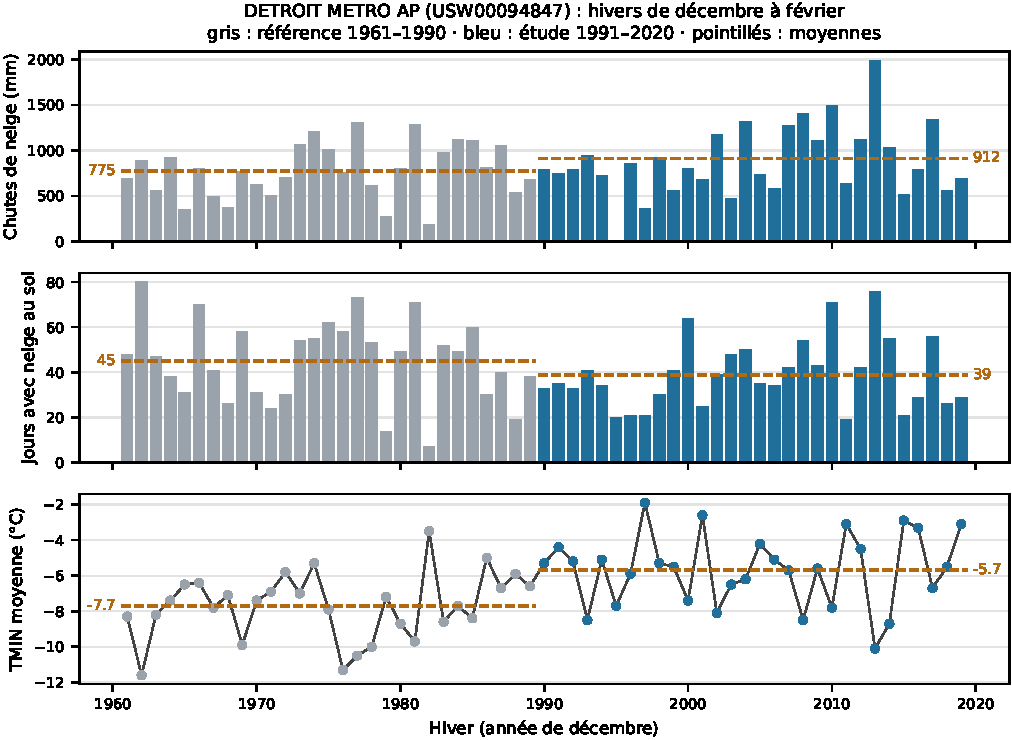
\includegraphics[width=0.8\textwidth]{assets/hivers_USW00094847.pdf}
  \caption{Hivers (décembre--février) à Detroit Metro, calculés par F1. Les hivers qui ne respectent pas la règle 3/5 sont omis.}
  \label{fig:hivers-detroit}
\end{figure}

\paragraph{Et aujourd'hui~?}
Les hivers 2020--21 à 2024--25, importés après coup par F5, prolongent la courbe. À Detroit Metro, ils comptent 34 jours de neige au sol en moyenne, contre 46 pendant les hivers d'enfance~; 2023--24 n'en a que 16. Et pour la première fois, la neige tombée passe elle aussi sous la normale~: 682~mm contre 775. Cinq hivers ne font pas une tendance, mais ils suggèrent la suite~: après une neige qui ne tient plus, une neige qui tombe moins.

\paragraph{Autant de neige, mais elle tient moins.}
Une station ne fait pas une région. Sur les 38 stations du Michigan qui mesurent à la fois la neige tombée et la neige au sol sur les deux périodes, la neige tombée ne bouge pas (1\,545 puis 1\,554~mm par hiver). Le nombre de jours de neige au sol passe pourtant de 73 à 67, soit 4,75 jours par 10~cm de neige au lieu de 5,28~: une baisse de 10~\%, observée à 27 stations sur 38. Les fortes chutes, elles, augmentent~: sur 64 stations, F2 compte 11~\% de jours de plus de 15~cm par an. L'hiver du Michigan n'est pas moins neigeux, il est moins durable.

\paragraph{Le sud de l'Allemagne perd plus vite.}
À l'échelle des zones, F3 compare chaque mois d'hiver de 1991--2020 à sa normale 1961--1990. Le Michigan perd 8~\% de ses jours de neige au sol (environ 6 jours par hiver) pour un réchauffement de 1,4~°C des minimales. Le sud de l'Allemagne, qui ne se réchauffe que de 1,0~°C, en perd 27~\% (environ 12 jours), et la perte s'accélère~: $-22$~\% sur 1991--2005, $-32$~\% sur 2006--2020.

\paragraph{Pourquoi~: l'hiver allemand a franchi zéro.}
La réponse tient au point de départ. Sur 66 stations de chaque zone, la journée d'hiver moyenne du Michigan passe de $-5,7$ à $-4,6$~°C~: plus chaude, mais encore loin du dégel, avec 63~\% des jours sous $-2$~°C. Celle du sud de l'Allemagne passe de $-0,5$ à $+0,7$~°C~: elle a franchi le point de fusion, et la part des jours au-dessus de $+2$~°C est montée de 31 à 40~\%. Le même réchauffement fond plus de neige là où l'hiver était déjà au bord du zéro.

\paragraph{Ce qui pourrait nous tromper.}
L'objection la plus sérieuse est l'arrivée massive de stations bénévoles au Michigan après 2008~: comparer des moyennes sur toutes les stations reviendrait à comparer deux réseaux différents. Tous les chiffres de cette section portent donc sur les mêmes stations aux deux périodes. Nos propres choix de paramètres ne changent pas non plus la conclusion~: avec un seuil d'altitude à 600~m, des cases de 0,5° ou de 2°, ou 20 à 27 années exigées pour une normale, le sud de l'Allemagne perd toujours entre 27 et 31~\% de ses jours de neige au sol, le Michigan entre 7 et 8~\% (annexe~\ref{annexe:sensibilite}). Garder seulement les stations allemandes sous 600~m, plus proches de zéro, accentue même la perte. Restent deux limites que nous ne levons pas~: la façon de mesurer la neige a pu changer d'un observateur à l'autre, et aucun test de significativité n'a encore été fait.

\paragraph{Vérifié sans notre système.} Un script séparé (\texttt{scripts/verify\_independent.py}) relit les fichiers NOAA d'origine avec pandas, sans MongoDB ni notre code, et réapplique les règles à partir de leur définition. Il retrouve les 181 épisodes de chaleur de l'été 2003 que donne F2, identiques station par station et jour par jour, et les 180 mois d'hiver de F3 à 0,005 près, l'écart venant de nos arrondis~: $-7,9$~\% de jours de neige au sol au Michigan, $-27,0$~\% dans le sud de l'Allemagne, comme dans la section~\ref{sec:resultats}.
% TODO : test statistique (par exemple Mann-Whitney sur les hivers des deux périodes).
